\documentclass{article}

\usepackage{full page}
\usepackage{pdfpages}
\usepackage{graphicx}
\usepackage{float}
\usepackage{mdframed}
\usepackage{minted}
\usepackage{enumerate}


\usepackage{listings}
\lstset{language=Python}

\title{Profile Hidden Markov Models}
\author{Taylor Cathcart, Cam Setian, Kyle Tessier-Lavigne}

\begin{document}
\maketitle

\section{Introduction}

As the cost of genetic sequencing has dropped significantly over the past decade, there has become an abundance of unprocessed genetic data. Many different computational methods have been developed or adapted to look for patterns in sets of genetic sequences, including Hidden Markov Models, which are particularly useful for processing signals from noise. One of the first applications of HMMs was in speech recognition in the 70s, and since then, many uses have been found in biological sequence analysis, including gene prediction, sequence alignment, structural alignment, and more.\footnotemark[1] When we talk about problems concerning HMMs, we usually mean one of three things:
\begin{enumerate}
\item Evaluation: What is the probability that a particular sequence of emissions is the output of a HMM model?
\item Decoding: Given a sequence of emissions and a model, what is the most likely sequence of states that emitted the given sequence?
\item Training: Given a set of sequences and a model, find a model that best fits the emission sequences.
\end{enumerate}
In this report, we begin by attempting to train a model and then move on to solve the evaluation problem. We can then use this to create models based on families of sequences and cross-validate our model, as well as potentially use it to identify other sequences in the family.

\footnotetext[1]{Hidden Markov Models and their Applications in Biological Sequence Analysis. Current Genomics. Sep 2009; 10(6): 402-415}

\section{Hidden Markov Models}

A Hidden Markov Model describes the probabilistic relationship between a set of hidden (i.e. unobservable) states and a set of known observations. If one knows the probability of going from one state to another at each time interval (the transition probability), and the probability that a given observation will be expressed by each state (the emission probability), then given a sequence of observations, one should be able to use this model to predict the most likely sequence of states corresponding to those observations. For example, say two people, Ann and Bob, live far apart. Bob tells Ann what he did each day for a week. Ann, who lives far from Bob, doesn't know what the weather is like for Bob each day. However, Ann does know the probability that Bob will do a certain activity based on the weather where he lives. She also knows the probability that a rainy day will be followed by a sunny day, and vice-versa. Using this information (where the weather reprsents the unobservable state, and the activity represents the observation for that day), Ann should be able to figure out the most likely weather pattern for that week.
\begin{figure}[H]
\centering
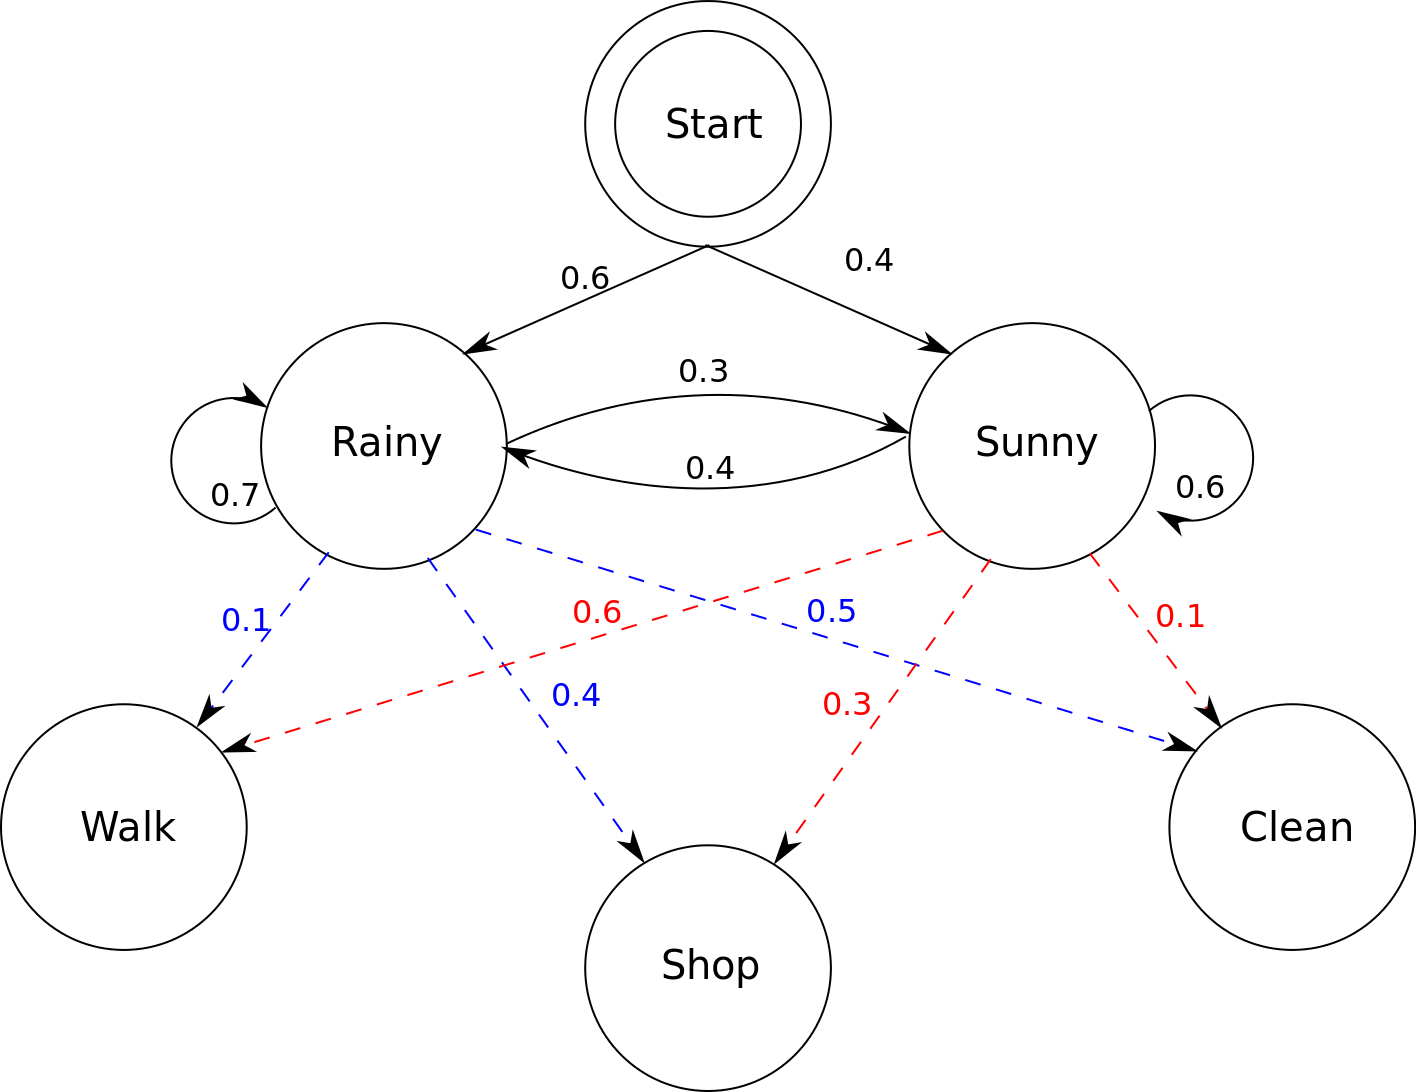
\includegraphics[width=.5\textwidth]{materials/HMMGraph.png}
\caption{Transition probabilities between states, and their emission probabilities for each observation\footnotemark[2]}
\end{figure}

\footnotetext[2]{http://en.wikipedia.org/wiki/File:HMMGraph.svg}

\section{Profile-Hidden Markov Models}

Profile-Hidden Markov Models are an adaptation of HMMs used to model genetic sequences. A profile-HMM consists of a sequence of match, insert, and delete states which span the length of the consensus sequence. A match corresponds to the expression of either a nucleotide (in the case of DNA sequencing) or an amino acid (in the case of protein sequencing). Insert and delete states correspond to the expression of a gap. 
\begin{figure}[H]
\centering
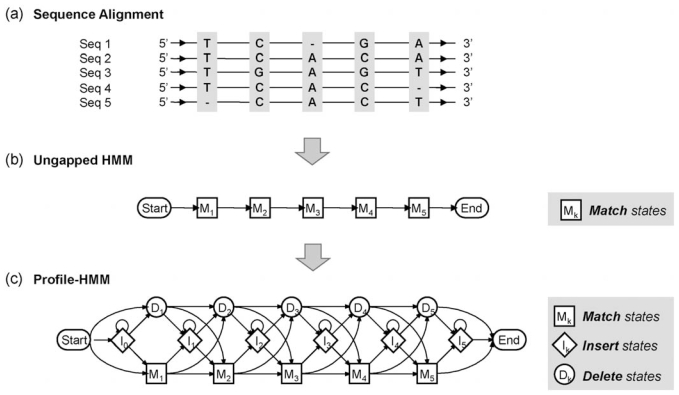
\includegraphics[width=.8\textwidth]{materials/profile-HMM.png}
\caption{profile-HMM\footnotemark[1]}
\end{figure}
Each position in the sequence is represented by one match state, one insert state, and one delete state. Aside from the insert states, a state may only transition to another state that is in the next sequential step in the sequence. Thus each position in the sequence (1 \ldots k) can be represented as $M_{1} I_{1} D_{1}, M_{2} I_{2} D_{2} \ldots M_{k} I_{k} D_{k}$. The probabilities of each state transitioning to each other valid state describes the set of transition probabilities for the model. Each match state contains a probability distribution for the alphabet of amino acids, describing the set of emission probabilities for that state.

\section{Methods}


\subsection{profile-HMM implementation}
The profile-HMM is first initialized with a start and end node (which do not correspond to the sequence itself), as well as transition probabilities using a pseudocount of 1 for each weight (scaled for insertions and deletions to 0.2). The actual profile itself is constructed in the ProfileHMM class

\subsection{Viterbi Scoring Algorithm}



\section{Application}
We had planned to test our profile-HMM using two different gene families taken from pfam, Cancer-associated gene protein 1 (CAGE1)\footnotemark[3] and Oesophageal cancer-related gene 4 (Augurin).\footnotemark[4] Using the smaller seed alignments for each family, which pfam used to assemble the family as a whole, we planned to train two separate models (one for each family). We would then compare our models to both their own sets and the opposite sets to confirm that our model was getting higher probability scores for its own family.

In order to compare against more established methods, we planned to build HMMs on the same seed multiple sequence alignments using HMMer, then run a search on pfam's database using those HMMs and compare to our own results.

Ideally we would have also been able to generate HMM logos based on our results. However, we ran into a lot of problems due to the formatting of HMM files, which has very sparse documentation. Because of this, we had trouble integrating and comparing our results with established methods.

\begin{figure}[H]
\centering
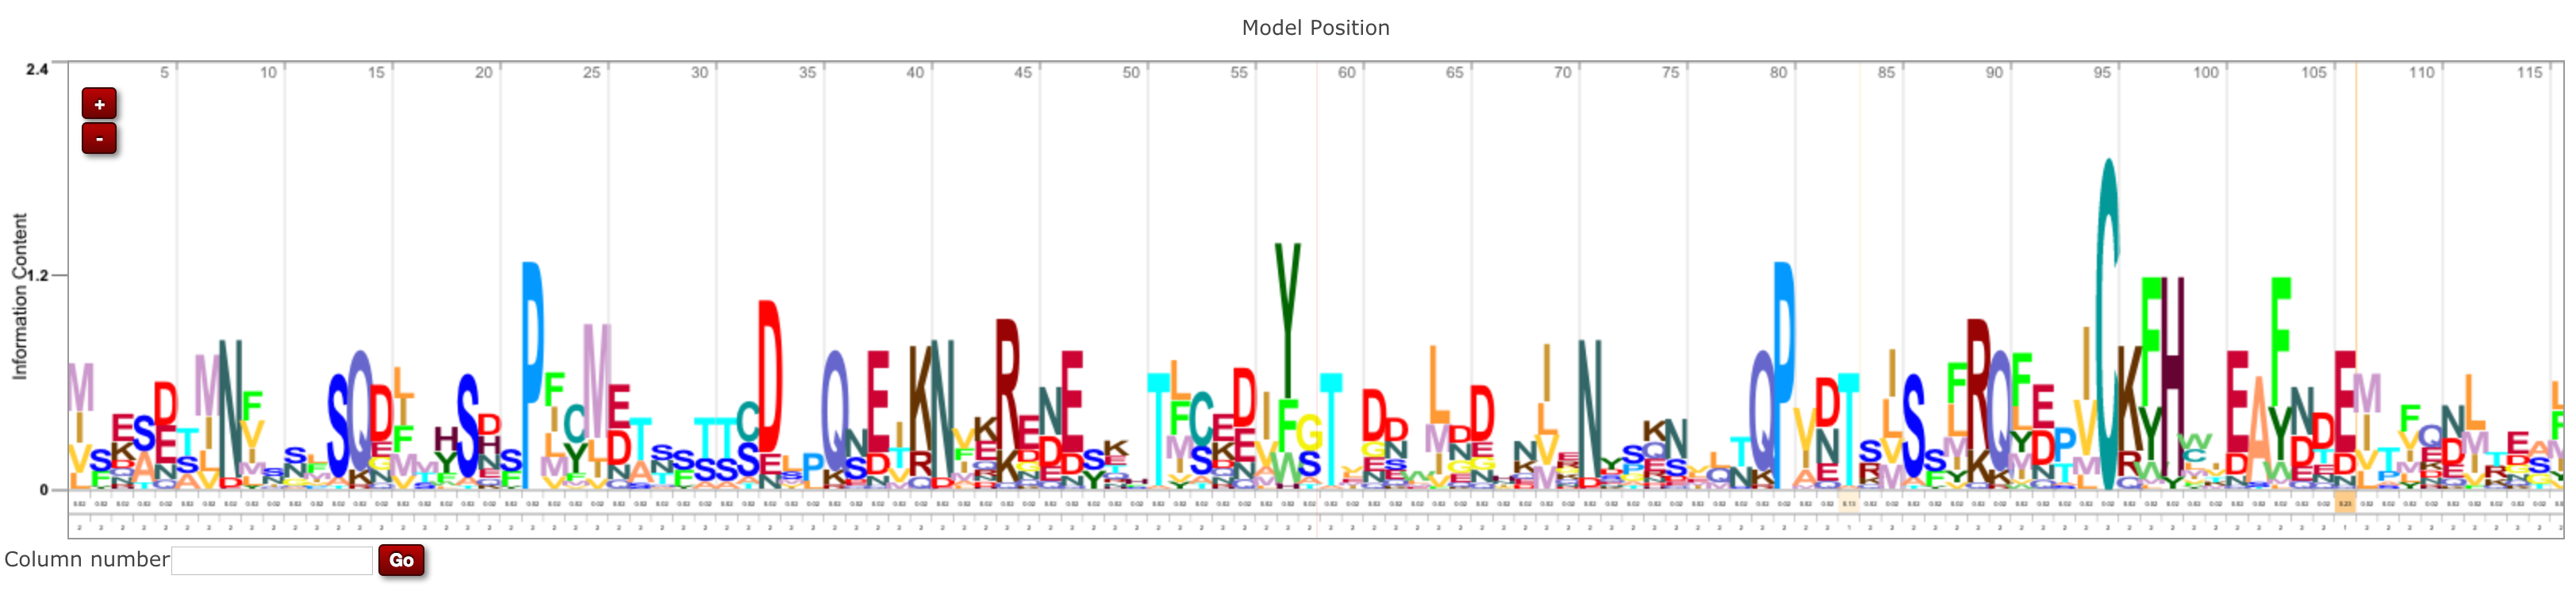
\includegraphics[width=1.0\textwidth]{materials/HMMerLogo.png}
\caption{HMMer logo generated from the PF15066 (CAGE1) Seed MSA}
\end{figure}



\footnotetext[3]{http://pfam.xfam.org/family/PF15066}
\footnotetext[4]{http://pfam.xfam.org/family/PF15187}

\section{Results}

While we weren't able to accomplish all of our goals, we were able to implement a training algorithm for profile-HMMs based on MSAs and also the forward-backward evaluation part of Baum-Welch. Attached is our output for the profile-HMM generated from the PF15187\_seed.txt MSA (in data/gen\_PF15187.hmm), which is too large to include in this report. PF15187.hmm is the pfam generated HMM for the same data set. It was difficult to interpret pfam's results without more information on the formatting of the data, and we feel that the differences in output are due to the varied structuring of the programs. We believe the maximization step failed because of an underflow error. The probabilities produced by the Forward-Backward algorithm approached zero due to the accumulation of rounding floating point errors. In the future, we would use a log-likelihood transformation to avoid this problem.


\section{Division of Labor}
As a whole, all members of the team were involved in the various aspects of this process. All three of us were involved in the research and planning of the project. Taylor worked mainly on the architecture of the profile-HMM, while Kyle focused on the training aspect of the algorithm. Cam took the lead on applications and Baum-Welch implementation. 



\end{document}